\documentclass[12pt, a4paper, notitlepage, oneside]{article}
\usepackage[english]{babel}
\usepackage[utf8]{inputenc} 
\usepackage{graphicx}
\usepackage{hyperref}
\usepackage{enumerate}
\usepackage{setspace}
%\singlespacing

\makeatletter

\newcommand{\linia}{\rule{\linewidth}{0.4mm}}

\renewcommand{\maketitle}{
\begin{titlepage}

    \vspace*{1cm}

    \begin{center}\small

    Warsaw University of Technology\\
    The Faculty of Electronics and Information Technology\\

    \end{center}

    \vspace{3cm}

     \begin{center}

    Data Mining (EDAMI)\\ Project Documentation

    \end{center}

    \noindent\linia

    \begin{center}

      \LARGE \textsc{\@title}

         \end{center}

     \noindent\linia

    \vspace{0.5cm}

    \begin{flushright}

    \begin{minipage}{5cm}

    \textit{\small Authors:}\\

    \normalsize \textsc{\@author} \par

    \end{minipage}

    \vspace{4cm}
    
 

     \end{flushright}

    \vspace*{\stretch{6}}

    \begin{center}

    \@date

    \end{center}

  \end{titlepage}
}

\makeatother

\title{Clustering based on density}

\author{Aleksandra Kurdo\\ Adam Stelmaszczyk}

\begin{document}

\maketitle


\onehalfspacing


\section*{Project task}
Implementation and experimental evaluation of DBSCAN~\cite{dbscan} and DENCLUE~\cite{denclue} algorithms. 

%\section*{Solution specification}

\section*{Data set}

For the experiments was chosen dataset with information about geometrical properties of kernels belonging to three different varieties of wheat: Kama, Rosa and Canadian (70 elements each, randomly selected). This dataset was found at the page of \textit{UC Irvine Machine Learning Repository}~\cite{dataset}. This set has seven, real-valued attributes, and includes 210 instances. \footnote{\url{http://archive.ics.uci.edu/ml/machine-learning-databases/00236/seeds_dataset.txt}}

\subsection*{Data set attribute information}


To construct the data, seven geometric parameters of wheat kernels were measured: 

\begin{itemize}
	\item area A, 
	\item perimeter P, 
	\item compactness C, 
	\item length of kernel, 
	\item width of kernel, 
	\item asymmetry coefficient 
	\item length of kernel groove. 
\end{itemize}

All of these parameters were real-valued continuous.


\section*{Algorithms description}
 
\subsection*{DBSCAN algorithm}

DBSCAN algorithm is relatively simple algorithm controlled with 2 parameters, namely EPS and MIN\_PTS. \cite{dbscan}
Basically, we are iterating over a set of unvisited points. If we found a core point (a point which has
at least MIN\_PTS in his Eps-neighbourhood), we are starting a new cluster. Looking at the neighbours 
of found core point we are trying to expand this new cluster as much as possible (basing on the Eps-neighbourhood).



\subsection*{DENCLUE algorithm}

DENCLUE algorithm is based on the idea that the influence of each data point can be modeled using a mathematical function (influence function). The overall density of the data space can be calculated as the sum of the influence function of all data points. Clusters can be determined mathematically by identifying density-attractors, which are the local maxima of the overall density function. The DENCLUE algorithm works in two steps:

\begin{enumerate}
	\item It is preclustering step, in which a map of the relevant portion of the data space is constructed. The map is used to speed up the calculation of the density function which requires to efficiently access neighboring portions of the data space. 
	
	\item It is the actual clustering step, in which the algorithm identifies the density-attractors and the corresponding density-attracted points.
\end{enumerate}

\section*{Implementation details}

As implementation language for the project Java was chosen. 
Data set is read from a text file, that located in program root directory, and a set of objects that represent points is generated. 
On this set DBSCAN and DENCLUE algorithms are run. 
Other arguments that algorithms need are declared directly in the program files. Whole program consists of five packages:

\begin{itemize}
	\item \texttt{algorithms} In this package abstract class ClusteringAlgorithm and inherited from it classes DBSCAN and DENCLUE are located. 

	\begin{figure}[!ht]
 	\centering
	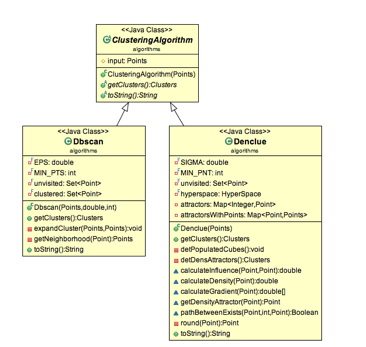
\includegraphics[width=0.8\textwidth]{images/algorithms_package.png}
 	\caption[]
	{Class diagram for algorithms package}
\label{algorithms}
	\end{figure}


	\item \texttt{structures} Here are located classes Cluster, Point and Points, that used simply to describe set of points and generated clusters. Diagram class is shown on the picture~\ref{structures}.

	\begin{figure}[!ht]
 	\centering
	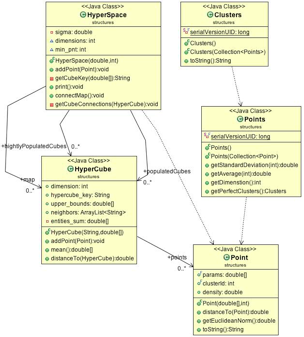
\includegraphics[width=0.8\textwidth]{images/structures_package.png}
 	\caption[]
	{Class diagram for structures package}
\label{structures}
	\end{figure}


	\item \texttt{scorer} This package consists of a class Scorer, that used to generate some statistics about created by algorithm clusters. Diagram class is shown on the picture~\ref{scorer}.

	\begin{figure}[!ht]
 	\centering
	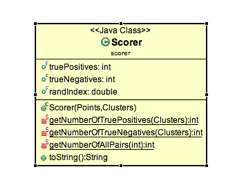
\includegraphics[width=0.6\textwidth]{images/scorer_package.png}
 	\caption[]
	{Class diagram for scorer package}
	\label{scorer}
	\end{figure}


	\item \texttt{visualizer} Used for the clusters visualization. Diagram class is shown on the picture~\ref{visualizer}.

	\begin{figure}[!ht]
 	\centering
	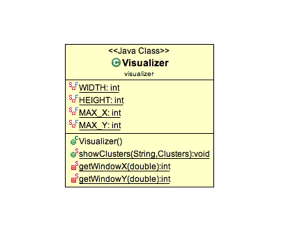
\includegraphics[width=0.6\textwidth]{images/visualizer_package.png}
 	\caption[]
	{Class diagram for visualizer package}
\label{visualizer}
	\end{figure}


	\item \texttt{main} Used for reading the data set from the file and executing algorithms. Diagram class is shown on the picture~\ref{main}.


	\begin{figure}[!ht]
 	\centering
	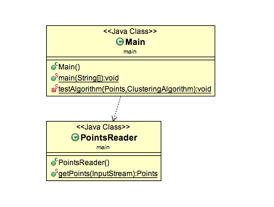
\includegraphics[width=0.8\textwidth]{images/main_package.png}
 	\caption[]
	{Class diagram for main package}
\label{main}
	\end{figure}

\end{itemize}



\section*{User guide}


Execute files from edami\_clustering.zip.


\noindent 
Create an empty java project in Eclipse IDE and import extracted files to it. 

\noindent 
Build the project using Eclipse.

\noindent 
To run the program please add execution rights to the run.sh file by typing in console: 
	chmod + ./run.sh 


\noindent 
Run program:
 ./run.sh


\cleardoublepage

\section*{Experimentation results and analysis}

As a result of execution DBSCAN and DENCLUE algorythms two sets of clusters are generated. This clusters are represented as points in 2D view as a set of points that belong to them (pictures~\ref{perfect}, ~\ref{dbscan}, ~\ref{denclue}). Each point represented as a number of it’s cluster. Data set attributes~\textit{area} and~\textit{asymmetry coefficient} are chosen as a dimensions of the view because of their standard deviation. 

\begin{figure}[!ht]
 	\centering
	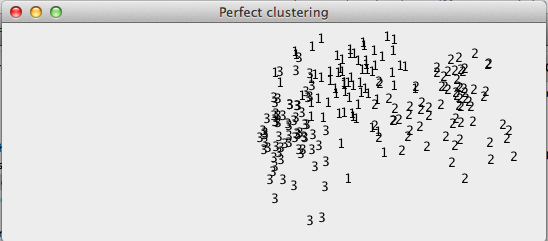
\includegraphics[width=0.6\textwidth]{images/perfect.png}
 	\caption[]
	{Perfect clustering}
	\label{perfect}
	\end{figure}

\begin{figure}[!ht]
 	\centering
	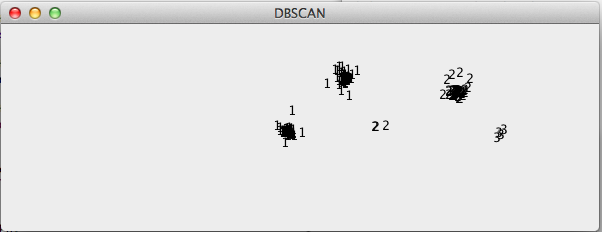
\includegraphics[width=0.6\textwidth]{images/dbscan.png}
 	\caption[]
	{Clustering made by DBSCAN algorithm}
	\label{dbscan}
	\end{figure}

\begin{figure}[!ht]
 	\centering
	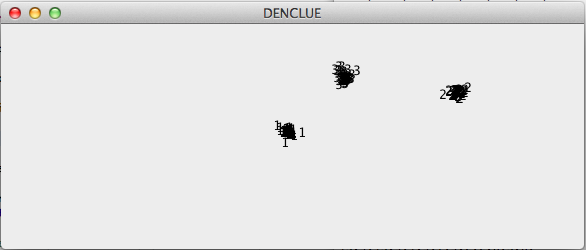
\includegraphics[width=0.6\textwidth]{images/denclue.png}
 	\caption[]
	{Clustering made by DENCLUE algorithm}
		\label{denclue}
	\end{figure}

Also some statistics for the running algorithms are shown, such as \textit{true positives}, \textit{true negatives} and \textit{rand index} (picture~\ref{result}).

\begin{figure}[!ht]
 	\centering
	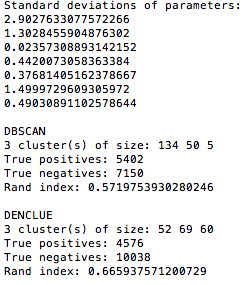
\includegraphics[width=0.35\textwidth]{images/results.png}
 	\caption[]
	{The output of the program}
		\label{result}
\end{figure}

Parameters for the algorithms were chosen experimentally. The best results were achieved using for DENCLUE and DBSCAN algorithms values near: 
$$sigma = 0.7, eps = 3$$

The comparison based on time of DENCLUE and DBSCAN algorithms is presented on figure~\ref{comparison_time}.

\begin{figure}[!ht]
 	\centering
	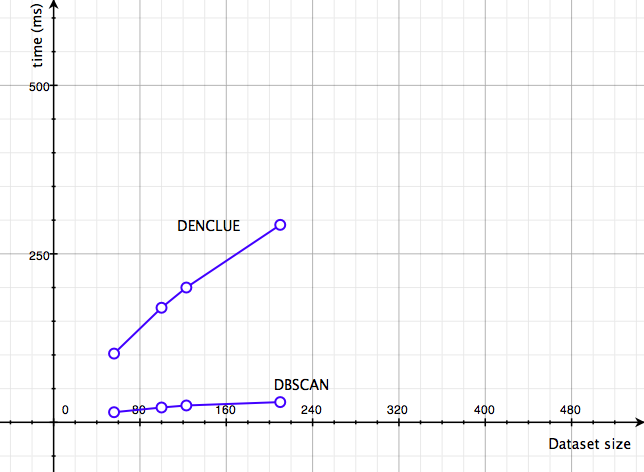
\includegraphics[width=0.7\textwidth]{images/comparison_time.png}
 	\caption[]
	{Comparison of DENCLUE and DBSCAN}
		\label{comparison_time}
\end{figure}

What can be seen from achieved by DBSCAN and DENCLUE algorithms results that they are quit different. Rand index for DENCLUE algorithm always was higher, what means that its results for this dataset are better. But on the other hand DENCLUE  algorithm was needed  more time than DBSCAN to do the same work. Should be noticed, that chosen dataset wasn't very big and this difference in time could be changed when algorithms would try to deal with really huge datasets. It can be assumed at the first sight, that for bigger dataset DENCLUE algorithm will be much more slower then DBSCAN, but it's not completely true. Time for DBSCAN algorithm in such situation will rise very quickly and on the other hand such elements in DENCLUE algorithm as dividing data points to cubes, take for big calculations only highly populated cubes ant other elements that were provided to faster the algorithm, will optimize it. And on the tested dataset DENCLUE algorithm dividing cubes for populated and highly populated wasn't a cause of some big decrease of considered cubes. 


\cleardoublepage


\section*{Conclusion}





%\url{http://archive.ics.uci.edu/ml/machine-learning-databases/00236/} 
\newpage

\bibliographystyle{plain}
\bibliography{references}
\end{document}